\section{U-Net Appendix}\label{s:unetAppendix}

\begin{figure}[H]
  \begin{center}
    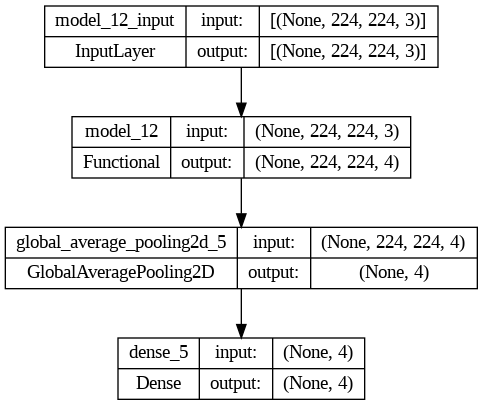
\includegraphics[width=0.35\textwidth]{unet/unetpp_model2.png}
  \end{center}
  \caption{U-Net++ model architecture}\label{fig:unetpp_model}
\end{figure}

Where \texttt{model\_12} is the U-Net++ model with EfficientNetB1 encoder. The Output Layer of \texttt{model\_12} is also used for the segmentation attempt to show what the model deems as the important parts of the image for the classification task.

\subsection{Segmentation Algorithm}\label{ss:segmentationAlgorithm}

\begin{algorithm}[H]
\caption{Image Prediction and Visualization with Mask Overlay}\label{alg:unet_visualization}
\begin{algorithmic}[1]
\State \textbf{Define} class names: $\texttt{classes} = \{\text{glioma}, \text{meningioma}, \text{notumor}, \text{pituitary}\}$
\State \textbf{Get} predictions from the U-Net model: $\texttt{predictions\_model\_2} \leftarrow \texttt{model.layers[0].predict(test\_generator)}$
\State \textbf{Get} prediction probabilities: $\texttt{predictions\_prob} \leftarrow \texttt{model.predict(test\_generator)}$
\State \textbf{Get} predicted classes: $\texttt{predictions} \leftarrow \arg\max(\texttt{predictions\_prob}, \text{axis}=1)$
\State \textbf{Set} threshold for binary mask: $\texttt{threshold} = 0.9$
\State \textbf{Create} binary mask: $\texttt{binary\_mask} \leftarrow (\texttt{predictions\_model\_2} > \texttt{threshold}).\texttt{astype(np.uint8)}$
\State \textbf{Initialize} displayed class counts: $\texttt{displayed\_classes\_counts} \leftarrow \{ \texttt{class\_name}: 0 \text{ for class\_name in classes} \}$
\State \textbf{Set} number of images per class to display: $\texttt{num\_images\_per\_class} = 2$
\State \textbf{Initialize} plot figure
\For{\texttt{each image in test\_generator}}
    \State \textbf{Get} actual class index and name: $\texttt{actual\_class\_index} \leftarrow \texttt{test\_generator.classes[i]}$, $\texttt{actual\_class\_name} \leftarrow \texttt{classes[actual\_class\_index]}$
    \If{\texttt{displayed\_classes\_counts[actual\_class\_name]} $\geq$ \texttt{num\_images\_per\_class}}
        \State \textbf{Continue to next image}
    \EndIf
    \State \textbf{Load} original image
    \State \textbf{Reshape} binary mask to match original image shape: $\texttt{reshaped\_binary\_mask} \leftarrow \texttt{binary\_mask[i][:, :, 0]}$
    \State \textbf{Overlay} mask on original image
    \State \textbf{Get} predicted class name: $\texttt{predicted\_class\_name} \leftarrow \texttt{classes[predictions[i]]}$
    \State \textbf{Plot} original image and overlayed mask
    \State \textbf{Update} displayed class counts: $\texttt{displayed\_classes\_counts[actual\_class\_name]} \leftarrow \texttt{displayed\_classes\_counts[actual\_class\_name]} + 1$
    \If{\texttt{all counts in displayed\_classes\_counts} $\geq$ \texttt{num\_images\_per\_class}}
        \State \textbf{Break} the loop
    \EndIf
\EndFor
\State \textbf{Display} plot with tight layout
\end{algorithmic}
\end{algorithm}

\subsection{Additional Segmentation Results}

\begin{figure}[H]
  \centering
  \begin{subfigure}[b]{0.23\textwidth}
    \centering
    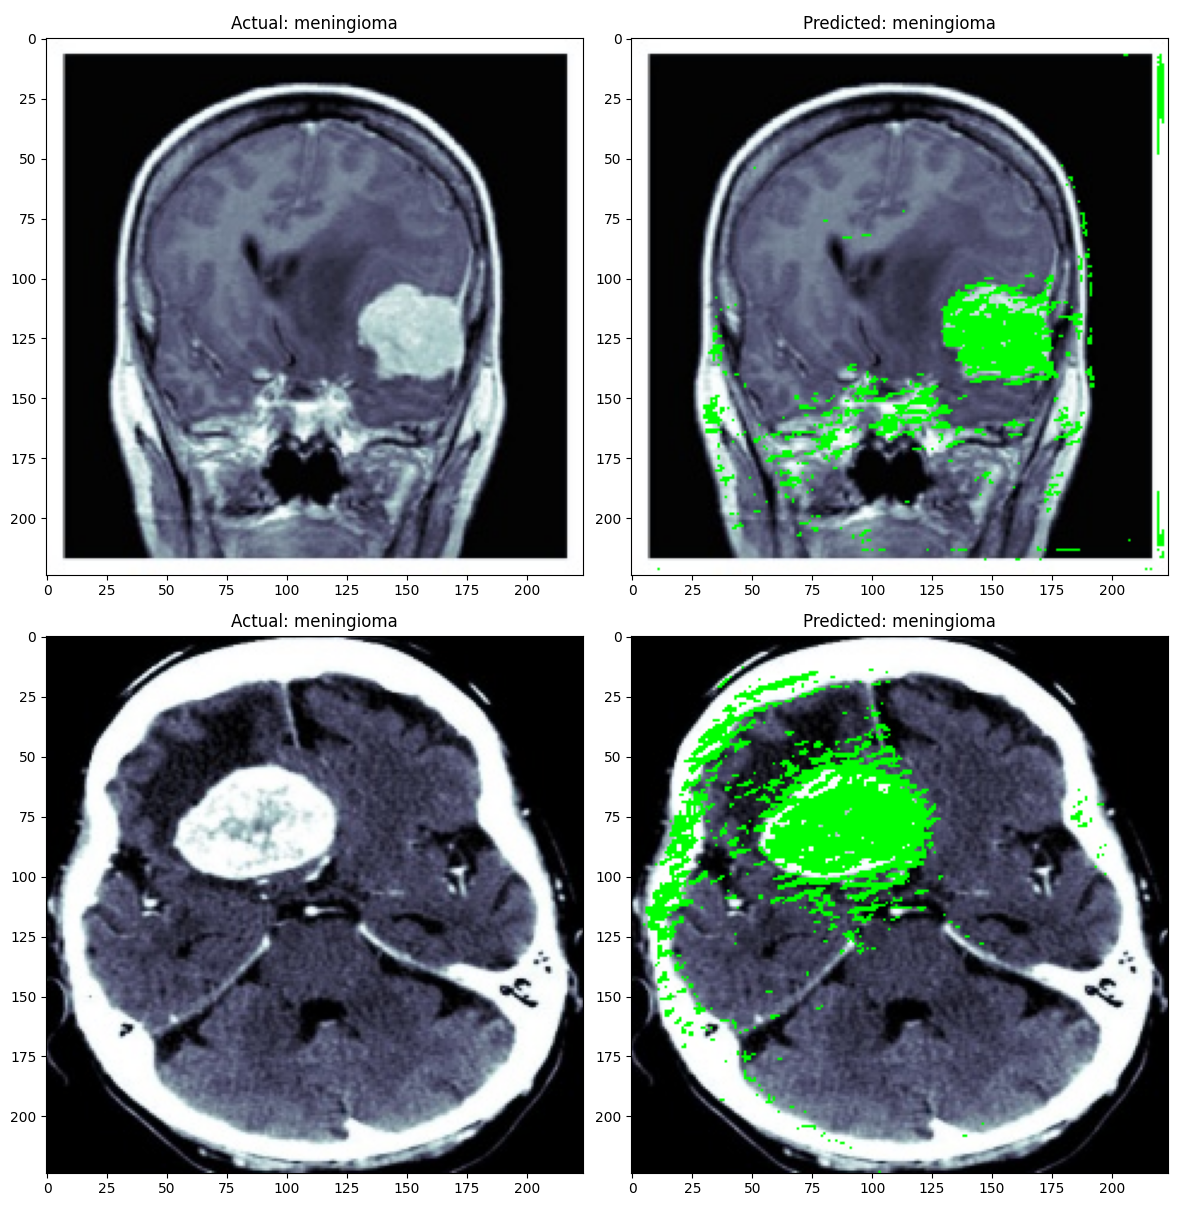
\includegraphics[width=\textwidth]{unet/evaluation/meningioma_1.png}
  \end{subfigure}
  \hfill
  \begin{subfigure}[b]{0.23\textwidth}
    \centering
    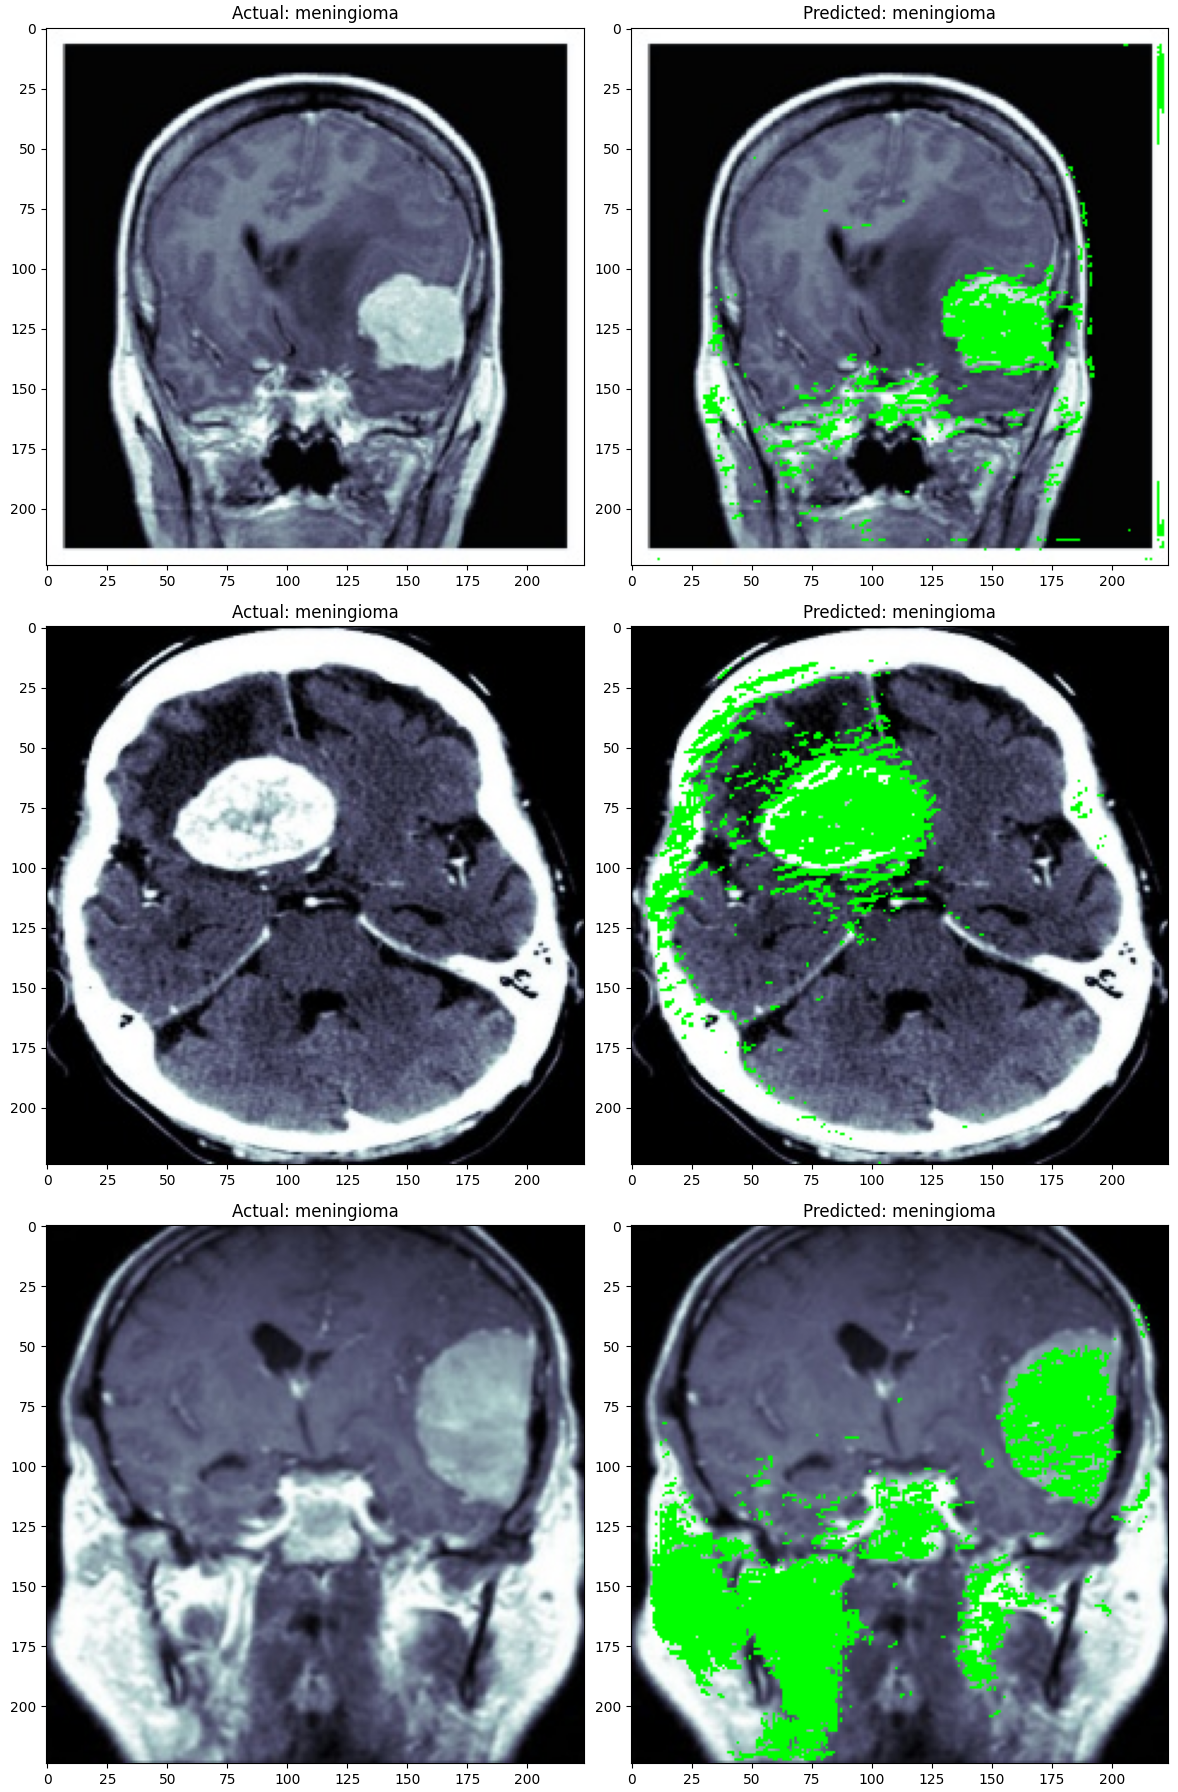
\includegraphics[width=\textwidth]{unet/evaluation/meningioma_2.png}
  \end{subfigure}
  \hfill
  \begin{subfigure}[b]{0.23\textwidth}
    \centering
    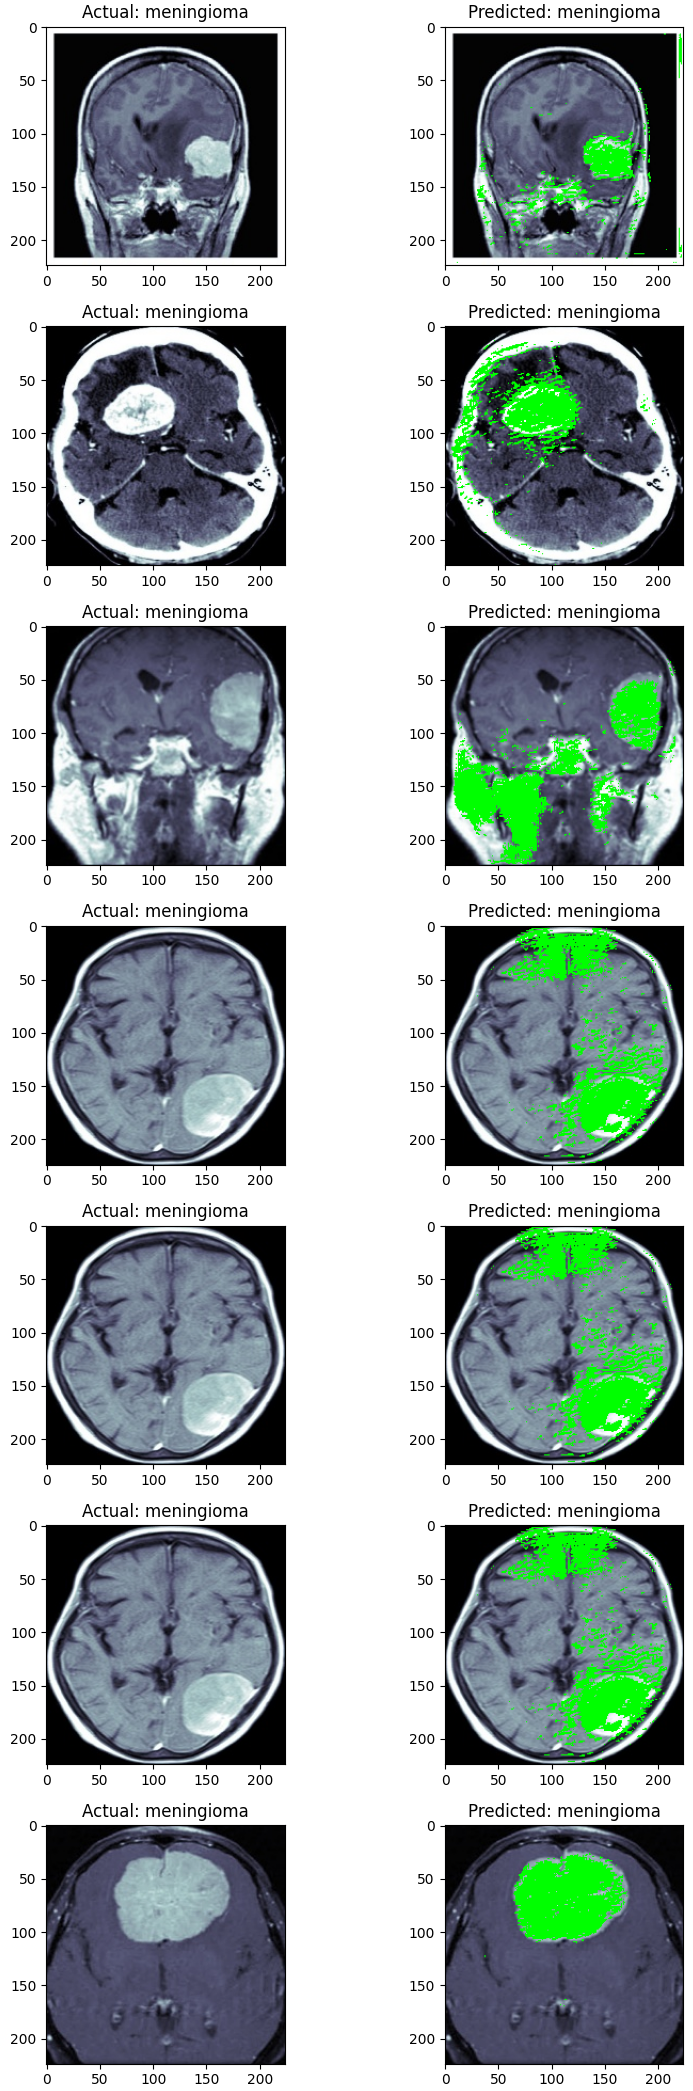
\includegraphics[width=\textwidth]{unet/evaluation/meningioma_3.png}
  \end{subfigure}
  \hfill
  \begin{subfigure}[b]{0.23\textwidth}
    \centering
    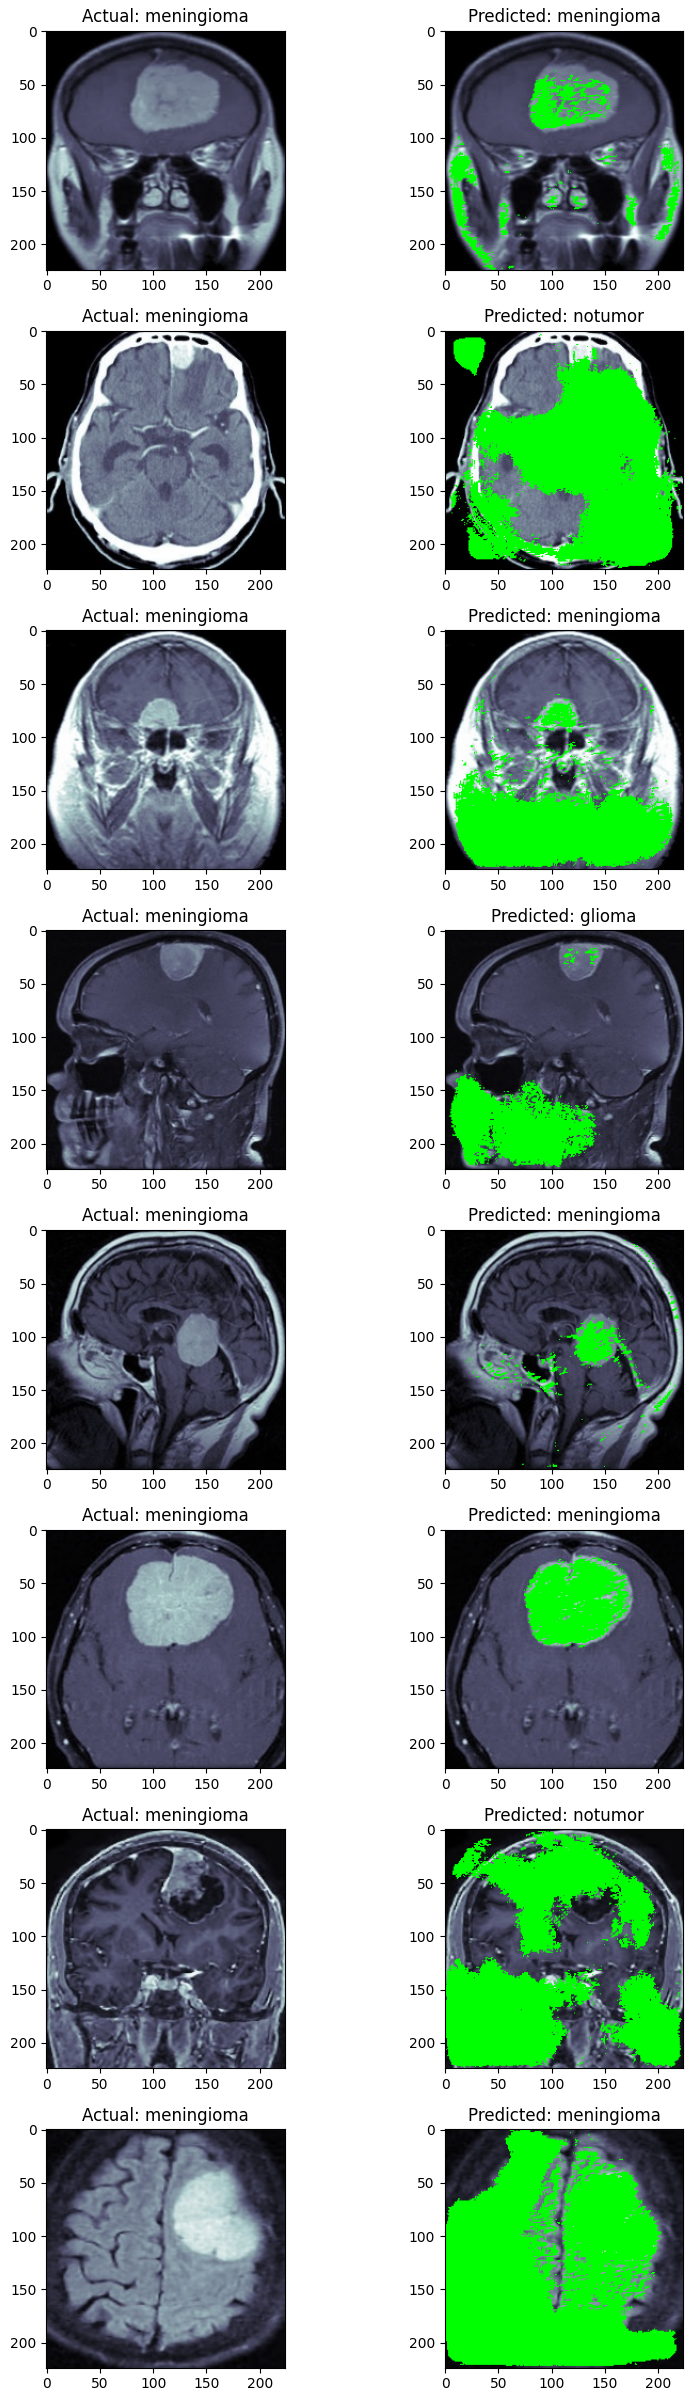
\includegraphics[width=\textwidth]{unet/evaluation/meningioma_4.png}
  \end{subfigure}
  \caption{Additional Segmentation Results for Menigioma}
  \label{fig:additional_malignoma_segmentation}
\end{figure}

Notice that the segmentation results are not perfect, but they are able to capture the general shape of the tumor. Some images that are predicted to not be part of the meningioma are also highlighted, since they are predicted to be part of another tumor.

\subsection{Jupyter Notebook}

\includepdf[
    %% Include all pages of the PDF
    pages=-,
    %% make this page have the usual page style
    %% (you can change it to plain etc). By default pdfpages
    %% sets the pagecommand to \pagestyle{empty}
    pagecommand={\pagestyle{headings}},  
    %% Add a "section" entry to the ToC with the heading
    %% "Quilling Shapes" and the label "sec:shapes"
    %addtotoc={1,section,1,Quilling Shapes,sec:shapes}
    ]
%% The pdf file itself
{unet.pdf}

